\documentclass{article}     
\usepackage{geometry}
\geometry{left=2.5cm,right=2.5cm,top=2.5cm,bottom=2.5cm}
\usepackage{graphicx}
\usepackage{float}
\usepackage{bm}
\usepackage{amsmath}
\usepackage{amsfonts}
\usepackage{amssymb}
\usepackage{newtxtext,newtxmath} 
\usepackage{setspace}
\usepackage{subfigure}
\usepackage{indentfirst}
\makeatletter
\newcommand{\bsf}[1]{\boldsymbol{\mathsf{#1}}}
\newcommand{\hb}[1]{\hat{\bsf{#1}}}
\DeclareMathOperator{\sign}{sign}


\makeatother
\setstretch{1.2}
\usepackage{tensor}
\usepackage{hyperref}
\usepackage{xcolor}
\usepackage[right]{showlabels}


\author{Wenqiang Fang} 
\title{Notes on derivation of governing equation of Elastica}
\date{}
\begin{document}
\maketitle

\section{Unit tangent vector and normal vector}

We assume that the position vector of a point is given by
\begin{equation}
\bsf{r}(s) = x_1(s) \hat{\bsf{e}}_1 + x_2(s) \hat{\bsf{e}}_2.	
\end{equation}	

\subsection{Unit tangent vector}
According to the definition of tangent vector (refer to \href{https://en.wikipedia.org/wiki/Frenet-Serret\_formulas}{Frenet-Serret formulas}), we have 
\begin{equation}
\label{eq:rprime}
\bsf{T}(s) = \frac{d \bsf{r}(s)}{d s} = x_1'(s) \hat{\bsf{e}}_1 + x_2'(s) \hat{\bsf{e}}_2.
\end{equation}

The norm of $\bsf{T}(s)$ is 
\begin{equation}
||\bsf{T}(s)|| = \left( x_1'(s)^2  + x_2'(s)^2  \right)^{1/2}.
\end{equation}

From in-extensibility of the beam, we have
\begin{equation}
\label{eq:in-extensibility}
 \left( x_1'(s)^2  + x_2'(s)^2  \right)^{1/2} = 1,
\end{equation}
which means $||\bsf{T}(s)||  = 1$. Thus we have the unit tangent vector
\begin{equation}
\label{eq:TUnit}
 \hat{\bsf{T}}(s) = \frac {\bsf{T}(s)} {||\bsf{T}(s)||} = \bsf{T}(s) = \bsf{r}'(s).
\end{equation}

\subsection{Unit normal vector}

The unit normal vector (refer to \href{https://en.wikipedia.org/wiki/Frenet-Serret\_formulas}{Frenet-Serret formulas}) is defined as
\begin{align}
\hat{\bsf{N}}(s) & =  \frac{d \bsf{T}(s)}{d s} \left|\left|\frac{d \bsf{T}(s)}{d s}\right|\right|^{-1}  \\
& =  \frac{x_1''(s) \hat{\bsf{e}}_1 + x_2''(s) \hat{\bsf{e}}_2}{(x_1''^2+ x_2''^2)^{1/2}} .
\end{align}

We take derivative of the in-extensibility condition~\eqref{eq:in-extensibility} and get
\begin{equation}
x_1' x_1'' + x_2' x_2'' = 0.
\end{equation}
Assuming that $x_1' = \cos(\theta)$ and $x_2' = \sin(\theta)$, we have
\begin{align}
x_1''(s) &= -\sin(\theta(s)) \theta'(s),\\
x_2''(s) &= \cos(\theta(s)) \theta'(s),\\
x_1''(s)^2 + x_2''(s)^2 &=  \theta'(s)^2 .
\end{align}
Therefore, the unit normal vector can be expressed as function of $\theta(s)$ as
\begin{equation}
\label{eq:NUnit}
\hat{\bsf{N}}(s)  = \sign\left[\theta'(s)\right] \left(-\sin(\theta(s))\hb{e}_1 + \cos(\theta(s))\hb{e}_2 \right).
\end{equation}

\section{Traction vector}

The traction vector $\bsf{t} (\bsf{\xi} (s))$ on position $\bsf{\xi} (s)$ of the beam can be returned as:
\begin{equation}
\bsf{t} (\bsf{\xi}(s)) = t_1 (\bsf{\xi}(s)) \hat{\bsf{T}}(s) + t_2 (\bsf{\xi}(s)) \hat{\bsf{N}}(s).
\end{equation}
where $\bsf{\xi} (s) = \xi \hat{\bsf{T}}(s) + \eta \hat{\bsf{N}}(s) + \zeta \hat{\bsf{B}}(s)$ and 
\begin{equation}
\hat{\bsf{B}}(s) = \hat{\bsf{T}}(s) \times \hat{\bsf{N}} (s) = \sign\left[\theta'(s)\right] \hb{e}_3,
\end{equation}
is called the binormal unit vector, $t_1(\bsf{\xi}(s))$ and $t_2(\bsf{\xi}(s))$ are the tangent and normal components of $\bsf{t} (\bsf{\xi}(s)) $, respectively.

We take integration on $\bsf{t} (\bsf{\xi}(s))  $ over cross section $\mathcal{A}(s)$
\begin{align}
\int_{\mathcal{A}(s)}  \bsf{t} (\bsf{\xi}(s)) \, dA  &
= \hat{\bsf{T}}(s) \int_{\mathcal{A}(s)} t_1 (\bsf{\xi}(s)) \, dA  
+ \hat{\bsf{N}}(s) \int_{\mathcal{A}(s)} t_2 (\bsf{\xi}(s)) \, dA  \\ &  
= V(s) \hat{\bsf{N}}(s)  +  T(s) \hat{\bsf{T}}(s),
\end{align}
where $V(s): = \int_{\mathcal{A}(s)}  t_2 (\bsf{\xi}(s)) \, dA $, $T(s) := \int_{\mathcal{A}(s)}  t_1 (\bsf{\xi}(s)) \, dA$. 


\begin{figure}[H]
\centering 
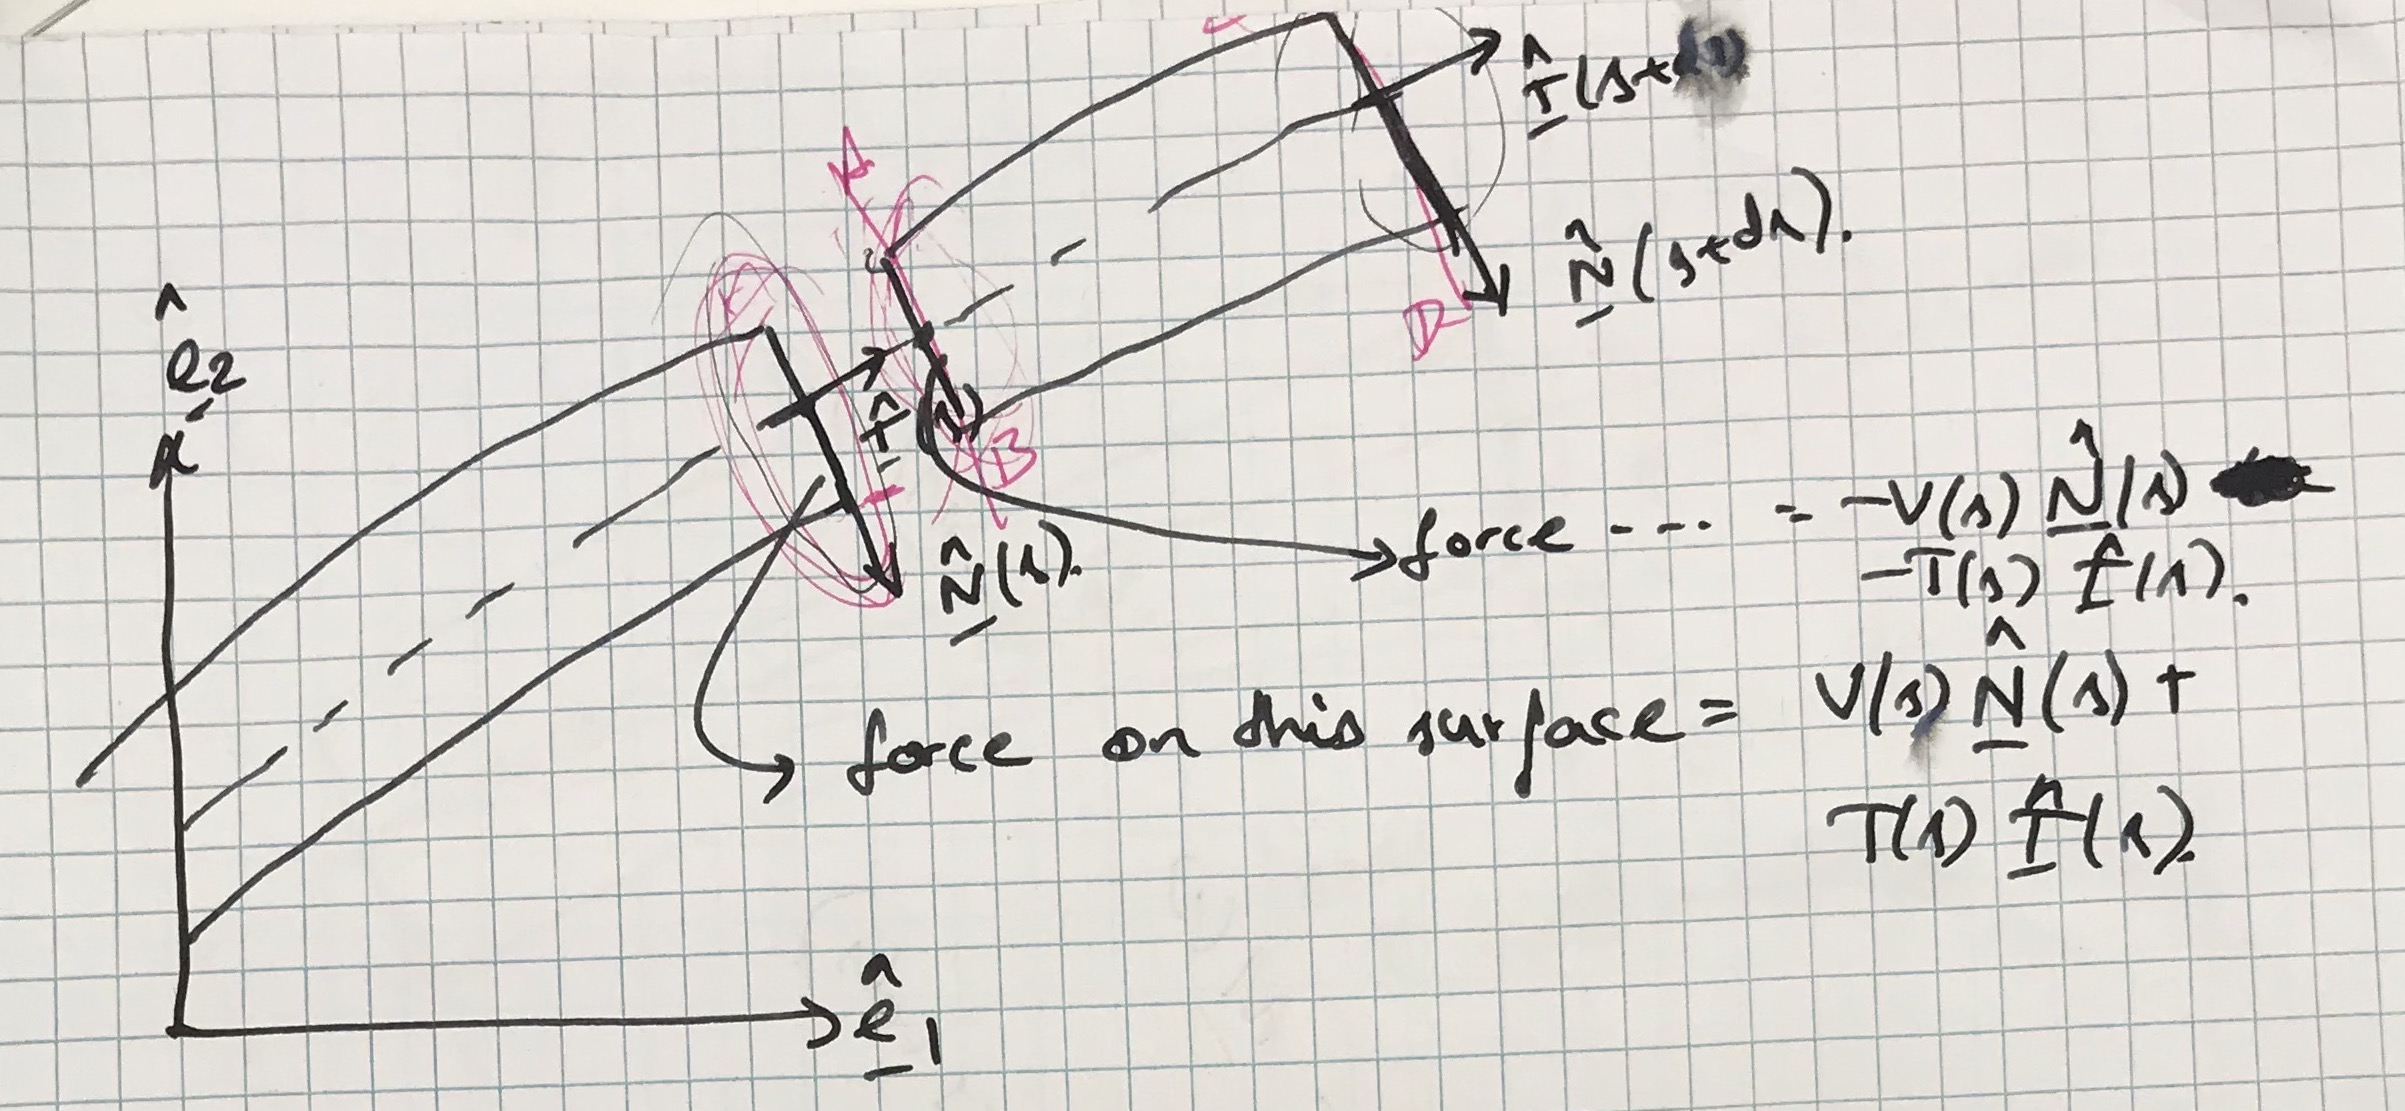
\includegraphics[width=0.7\textwidth]{Figures/Schematic.jpg}
\caption{Schematic of the beam}
\label{fig:schematic}
\end{figure}

The tractions acting on the surface  A-B (see Fig.~\ref{fig:schematic}) is 
\begin{equation}
-\bsf{t}(\bsf{\xi}(s))  = \bsf{\sigma} (s ) \left(-\hat{\bsf{T}}(s) \right) = - t_1 (\bsf{\xi}(s)) \hat{\bsf{T}}(s) - t_2 (\bsf{\xi}(s)) \hat{\bsf{N}}(s).
\end{equation}


\section{Moment on a cross section}

We compute the moment $- \bsf{M}(s) $ over the cross section  A-B (see Fig.~\ref{fig:schematic}) at $s$ is given by
\begin{align}
-\bsf{M} (s) & =   \int_{\mathcal{A}(s)} \bsf{\xi}(s) \times \left(-\bsf{t}(\bsf{\xi}(s))\right)  \, dA \\
			& =   \int_{\mathcal{A}(s)} \left( \xi \hat{\bsf{T}}(s) + \eta \hat{\bsf{N}}(s) + \zeta \hat{\bsf{B}}(s)\right) \times
			\left( - t_1(\bsf{\xi}(s)) \hat{\bsf{T}} (s)- t_2(\bsf{\xi}(s)) \hat{\bsf{N}}(s) \right) \, dA \\
			& =   \int_{\mathcal{A}(s)}  \left(- \xi  t_2\hb{B}(s) + \eta t_1(\bsf{\xi}(s)) \hb{B}(s) 
			     - \zeta t_1(\bsf{\xi}(s))\hb{N} (s)+ \zeta t_2(\bsf{\xi}(s))\bsf{t} (s) \right) \, dA \\
			& =   \int_{\mathcal{A}(s)}  \eta t_1(\bsf{\xi}(s)) \hb{B}(s)  \, dA,
			\label{eq:MomentExpression}
\end{align}
noting that in the local coordinate system, over cross section, $\xi = 0$. Because of symmetry, $\int_{\mathcal{A}(s)} \zeta t_1(\bsf{\xi}(s))\hb N (s)\, dA = \int_{\mathcal{A}(s)} \zeta t_2(\bsf{\xi}(s))\hb T(s) \, dA =  0$.

% \section*{Page 3\&4}
We can write Eqn.~\eqref{eq:MomentExpression} as 
\begin{align}
\bsf{M} (s)  &= M(s)   \hb{B}(s),\\
M(s) &=  -\int_{\mathcal{A}(s)}  \eta t_1(\bsf{\xi}(s))\, dA.
\label{eq:MomentScalar}
\end{align}

To build the link between moment and kinematic variables, we assume that the material of the beam is described by Hooke's Law. Therefore, 
\begin{equation}
\label{eq:hooke}
 t_1(\bsf{\xi}(s)) = E \epsilon_1(\bsf{\xi}(s)),
 \end{equation} 
 where $E$ is Young's modulus and $\epsilon_1(\bsf{\xi}(s)) $ is the normal strain on the cross section at $s$. We will derive $\epsilon_1(\bsf{\xi}(s)) $ in polar coordinate system, as shown in Fig.~\ref{fig:polar}.

The length of a fiber at $\eta  \hat{\bsf{N}}(s)$ is $(\rho(s)-\eta)$, where $\rho(s)$ is the local radius of curvature. The normal strain of this fiber is given by
\begin{equation}
\epsilon_1(\bsf{\xi}(s)) = \frac{(\rho(s)-\eta)d\theta  - \rho(s) d\theta}{\rho(s)d\theta} = -\frac{\eta}{\rho(s)}.
\end{equation}

We also know that $1/\rho(s)  = \kappa(s) = \left|\left|d \bsf{T}(s)/d s\right|\right|= \theta'(s) \sign\left[\theta'(s)\right]$. Thus
\begin{equation}
\label{eq:normalstrain}
\epsilon_1(\bsf{\xi}(s)) = -\eta \theta'(s) \sign\left[\theta'(s)\right].
\end{equation}

Substituting Eqns.~\eqref{eq:hooke} and~\eqref{eq:normalstrain} into Eqn.~\eqref{eq:MomentScalar}, we have that 
\begin{align}
M(s) &=  -\int_{\mathcal{A}(s)}  \eta E \epsilon_1(\bsf{\xi}(s))\, dA , \\
&=  E \theta'(s) \sign\left[\theta'(s)\right] \int_{\mathcal{A}(s)}  \eta^2  \, dA , \\
&=  E I \theta'(s) \sign\left[\theta'(s)\right] ,
\label{eq:MomentFinal}
\end{align}
where $I =  \int_{\mathcal{A}(s)}  \eta^2  \, dA $ is the second moment of inertia of the cross section.


\begin{figure}[H]
\centering 
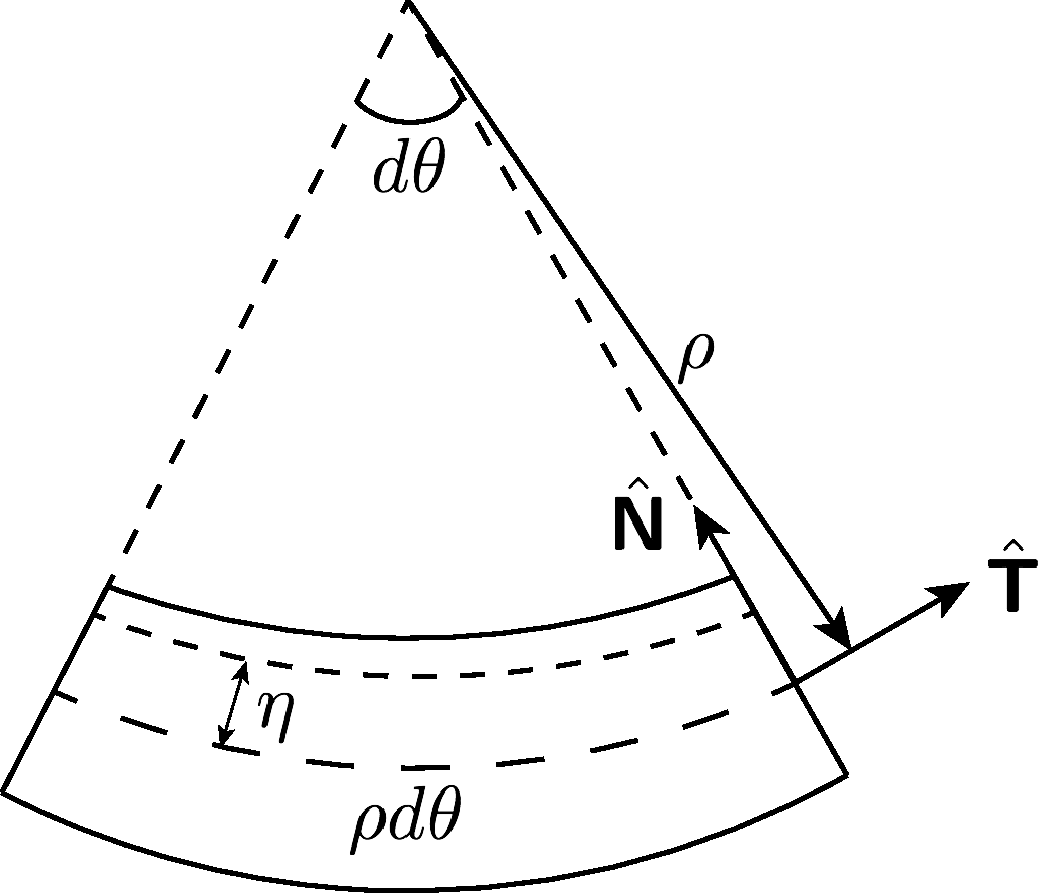
\includegraphics[width=0.4\textwidth]{Figures/sector.pdf}
\caption{Schematic of a infinitesimal section of a beam.}
\label{fig:polar}
\end{figure}



\section{Balance of force}

From force balance, we have equilibrium equation
\begin{equation}
\label{eq:balance}
\bsf{P} + V(s) \hat{\bsf{N}}  +  T(s) \hat{\bsf{T}} = \bsf{0},
\end{equation}
where $\bsf{P} = P_1 \hat{\bsf{e}}_1 +  P_2 \hat{\bsf{e}}_2 $ is the external applied force on beam's cross section.

We project the force balance equation~\eqref{eq:balance} in the direction of $\hat{\bsf{N}}$ to obtain
\begin{equation}
\label{eq:PV}
\bsf{P} \cdot \hat{\bsf{N}} + V(s)  = 0 .
\end{equation}

Recall that from Eqn.~\eqref{eq:NUnit}, we can simplify Eqn.~\eqref{eq:PV} as 
\begin{equation}
\label{eq:ForceBalance}
 \sign\left[\theta'(s)\right] \left(-\sin(\theta(s))P_1 + \cos(\theta(s))P_2\right) + V(s)  = 0 .
\end{equation}



\section{Balance of moment}


We apply balance of moment on the infinitesimal section of beam A-B-D-C (see Fig.~\ref{fig:schematic}),
\begin{equation}
\label{eq:BalanceofMoment}
-\bsf{M}(s) + \int_{\mathcal{A}(s+ds)} \Delta\bsf{r} \times \bsf{t}(\bsf{\xi}(s+ds)) \, dA +  \int_{\mathcal{A}(s+ds)}  \bsf{\xi} \times \bsf{t}(\bsf{\xi}(s+ds)) \, dA = 0, 
\end{equation}
where 
\begin{align}
\int_{\mathcal{A}(s+ds)} \Delta \bsf{r} \times \bsf{t}(\bsf{\xi}(s+ds)) \, ds 
&= \Delta\bsf{r} \times  \int_{\mathcal{A}(s+ds)}   \bsf{t}(\bsf{\xi}(s+ds)) \, ds  \\
&=  \Delta \bsf{r} \times (V(s+ds) \hb{N}(s+ds) + T(s+ds) \hb{N}(s+ds) ) \\
&=  \left(\bsf{r}'(s) ds + o(ds) \right) \times \left( \left(V(s)+V'(s)ds + o(ds) \right) \left(\hb{N}(s)+\hb{N}'(s)ds + o(ds) \right)  \right)\\
&+ \left(\bsf{r}'(s)ds + o(ds) \right) \times \left( \left(T(s)+T'(s)ds + o(ds) \right) \left(\hb{T}(s)+\hb{T}'(s)ds + o(ds) \right) \right) \\
&=  \bsf{r}'(s) ds \times \left(V(s) \hb{N}(s) + T(s)\hb{T}(s) + o(ds) \right)+ o(ds),
\label{eq:Moment2}
\end{align}
and 
\begin{align}
\int_{\mathcal{A}(s+ds)}  \bsf{\xi} \times \bsf{t}(\bsf{\xi}(s+ds)) \, dA 
& = \bsf{M}(s+ ds) \\
& = \bsf{M}(s) + \bsf{M}'(s)ds + o(ds).
\label{eq:Moment3}
\end{align}

Recall that from Eqn.~\eqref{eq:rprime} and~\eqref{eq:TUnit}, we have 
\begin{equation}
\bsf{r}'(s) = \hb{T}(s).
\end{equation}

Combing Eqns.~\eqref{eq:BalanceofMoment},~\eqref{eq:Moment2} and~\eqref{eq:Moment3}, we have
\begin{align}
& -\bsf{M}(s) +  \hb{T}(s) \times \left(V(s) \hb{N}(s) + T(s)\hb{T}(s) + o(ds) \right)+ \bsf{M}(s) + \bsf{M}'(s)ds + o(ds)\\
= & V(s) \hb{B}(s) + o(ds) + \bsf{M}'(s)ds + o(ds) \\
= & \left( V(s) \hb{B}(s) + \bsf{M}'(s) \right)ds + o(ds) \\
= & 0.
\end{align}

Thus we have 
\begin{equation}
V(s) \hb{B}(s)  = - \bsf{M}'(s) ,
\end{equation}
which is equivalently (assuming the sign of $\theta'(s)$ does not change, i.e., $\hb{B}(s)$ remain the same)
\begin{equation}
\label{eq:MomentBalance}
V(s)  = - M'(s) .
\end{equation}


\section{Final governing equation}


Combing force balance~\eqref{eq:ForceBalance} and moment balance~\eqref{eq:MomentBalance}, we have
\begin{equation}
 M'(s)  + \sign\left[\theta'(s)\right]  \left(P_1 \sin(\theta) - P_2 \cos(\theta) \right)= 0 .
\end{equation}

From Eqn.~\eqref{eq:MomentFinal}, we have
\begin{equation}
 E I \theta''(s) + \left(P_1 \sin(\theta) - P_2 \cos(\theta) \right)= 0 .
\end{equation}

\end{document}   